
\documentclass[letterpaper,11pt]{article}
\usepackage[utf8]{inputenc}
\usepackage[spanish]{babel}
\usepackage{mathtools}

\begin{document}

\title{Análisis de algoritmos iterativos y recursivos\\\large Actividad 2}
\author{Dagoberto Quevedo}
\maketitle

\begin{abstract}
En esta actividad se realiza realizar una implementación recursiva e iterativa de los siguientes algoritmos: (a) Búsqueda binaria, (b) Exponenciación entera y (c) Torres de Hanoi. Para cada implementación evaluar con distintas instancias su eficiencia en términos de tiempo de ejecución y se identifican las instancias que generan el peor caso.
\end{abstract}

\section{Exponenciación entera}

La exponenciación entera consiste en computar la potencia $a^b$, esto se deriva de una definición abreviada de la multiplicación siguiente $a^b=a\times a \dots^b \dots \times a$, donde $b$ es el número de veces que $a$ se multiplica a si mismo. En el caso de la exponenciación, cuando el componente $b$ de la operación es par se tiene que,
\begin{equation}
	a^b = [a \times \dots ^{b/2} \dots \times a] \times [a \times \dots ^{b/2} \dots \times a]  = a^{b/2} \times a^{b/2},
	%\dots \dots \times a \] \times \[a\times \dots  \dots \times a \]
\end{equation}
por lo cual, la definición recursiva de esta operación puede definirse como sigue,
\[
    a^b= 
\begin{cases}
    a^{b/2} \times a^{b/2}	,& \text{si } b> 0 \text{ y }  b \bmod 2 = 0, \\
    a\times a^{b-1}		,& \text{si } b> 0 \text{ y }  b \bmod 2 > 0, \\
    1					,& b > 0.
\end{cases}
\]
\subsection{Implementación y condiciones de experimentación}
Se realiza la implementación recursiva e iterativa de la operación en Python, la evaluación se realiza ejecutando una serie de instancias, en este caso cada instancia se define $a^{2^1} \dots a^{2^n}$, donde $a=1000$ y $n=25$, la ejecución se repite $k$ veces.

\subsection{Resultados}
El gráfico \ref{fig:ie} muestra los resultados del diseño experimental en el tiempo de computo expresado en escala logarítmica, el eje vertical expresa el valor de $n$ que define la instancia $a^{2^n}$.

\begin{figure}[h!]
  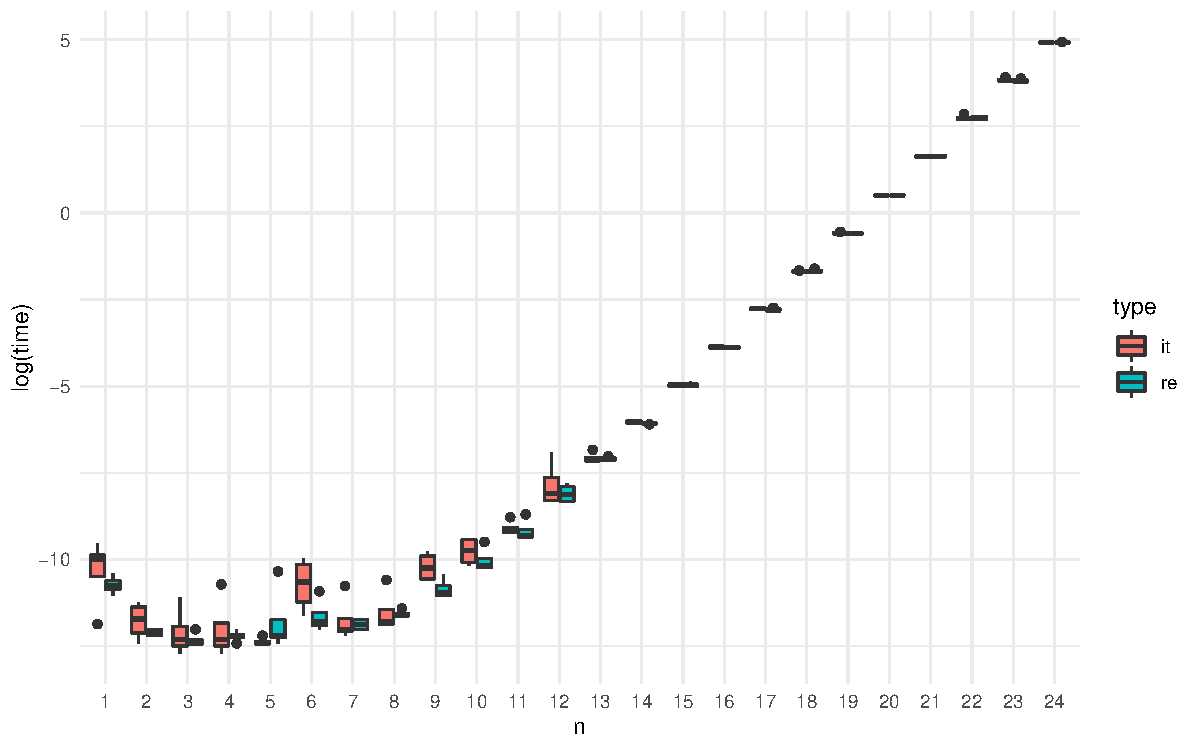
\includegraphics[width=\linewidth]{ie.pdf}
  \caption{Resultados del diseño experimental con $k$ ejecuciones para cada tipo de implementación e instancia de prueba}
  \label{fig:ie}
\end{figure}

Los resultados muestran que no existe evidencia suficiente a partir del tiempo de computo para concluir que una implementación es mejor que otra, esto debido a que el número de operaciones requerido para ambas implementaciones es aproximadamente igual.


\end{document}
